% "{'classe':('PSI'),'chapitre':'tec_3d','type':('td'),'titre':'Robot de dépose de fibres optiques', 'source':'oncours Mines Ponts - PSI 2004','comp':('C1-05','C2-08'),'corrige':True}"
%\setchapterimage{bandeau}

\chapter*{TD \arabic{cptTD} \\ 
Robot de dépose de fibres optiques \ifnormal $\star$ \else \fi \iftdifficile $\star\star\star$ \else \fi -- \ifprof Corrigé \else Sujet \fi}
\addcontentsline{toc}{section}{TD \arabic{cptTD} : Robot de dépose de fibres optiques \ifnormal $\star$ \else \fi \iftdifficile $\star\star\star$ \else \fi  -- \ifprof Corrigé \else Sujet \fi}

\iflivret \stepcounter{cptTD} \else
\ifprof  \stepcounter{cptTD} \else \fi
\fi

\setcounter{question}{0}
\marginnote{Concours Mines Ponts -- PSI 2004.}
\marginnote{
\UPSTIcompetence[2]{C1-05}
\UPSTIcompetence[2]{C2-08}}


\begin{marginfigure} [2cm]
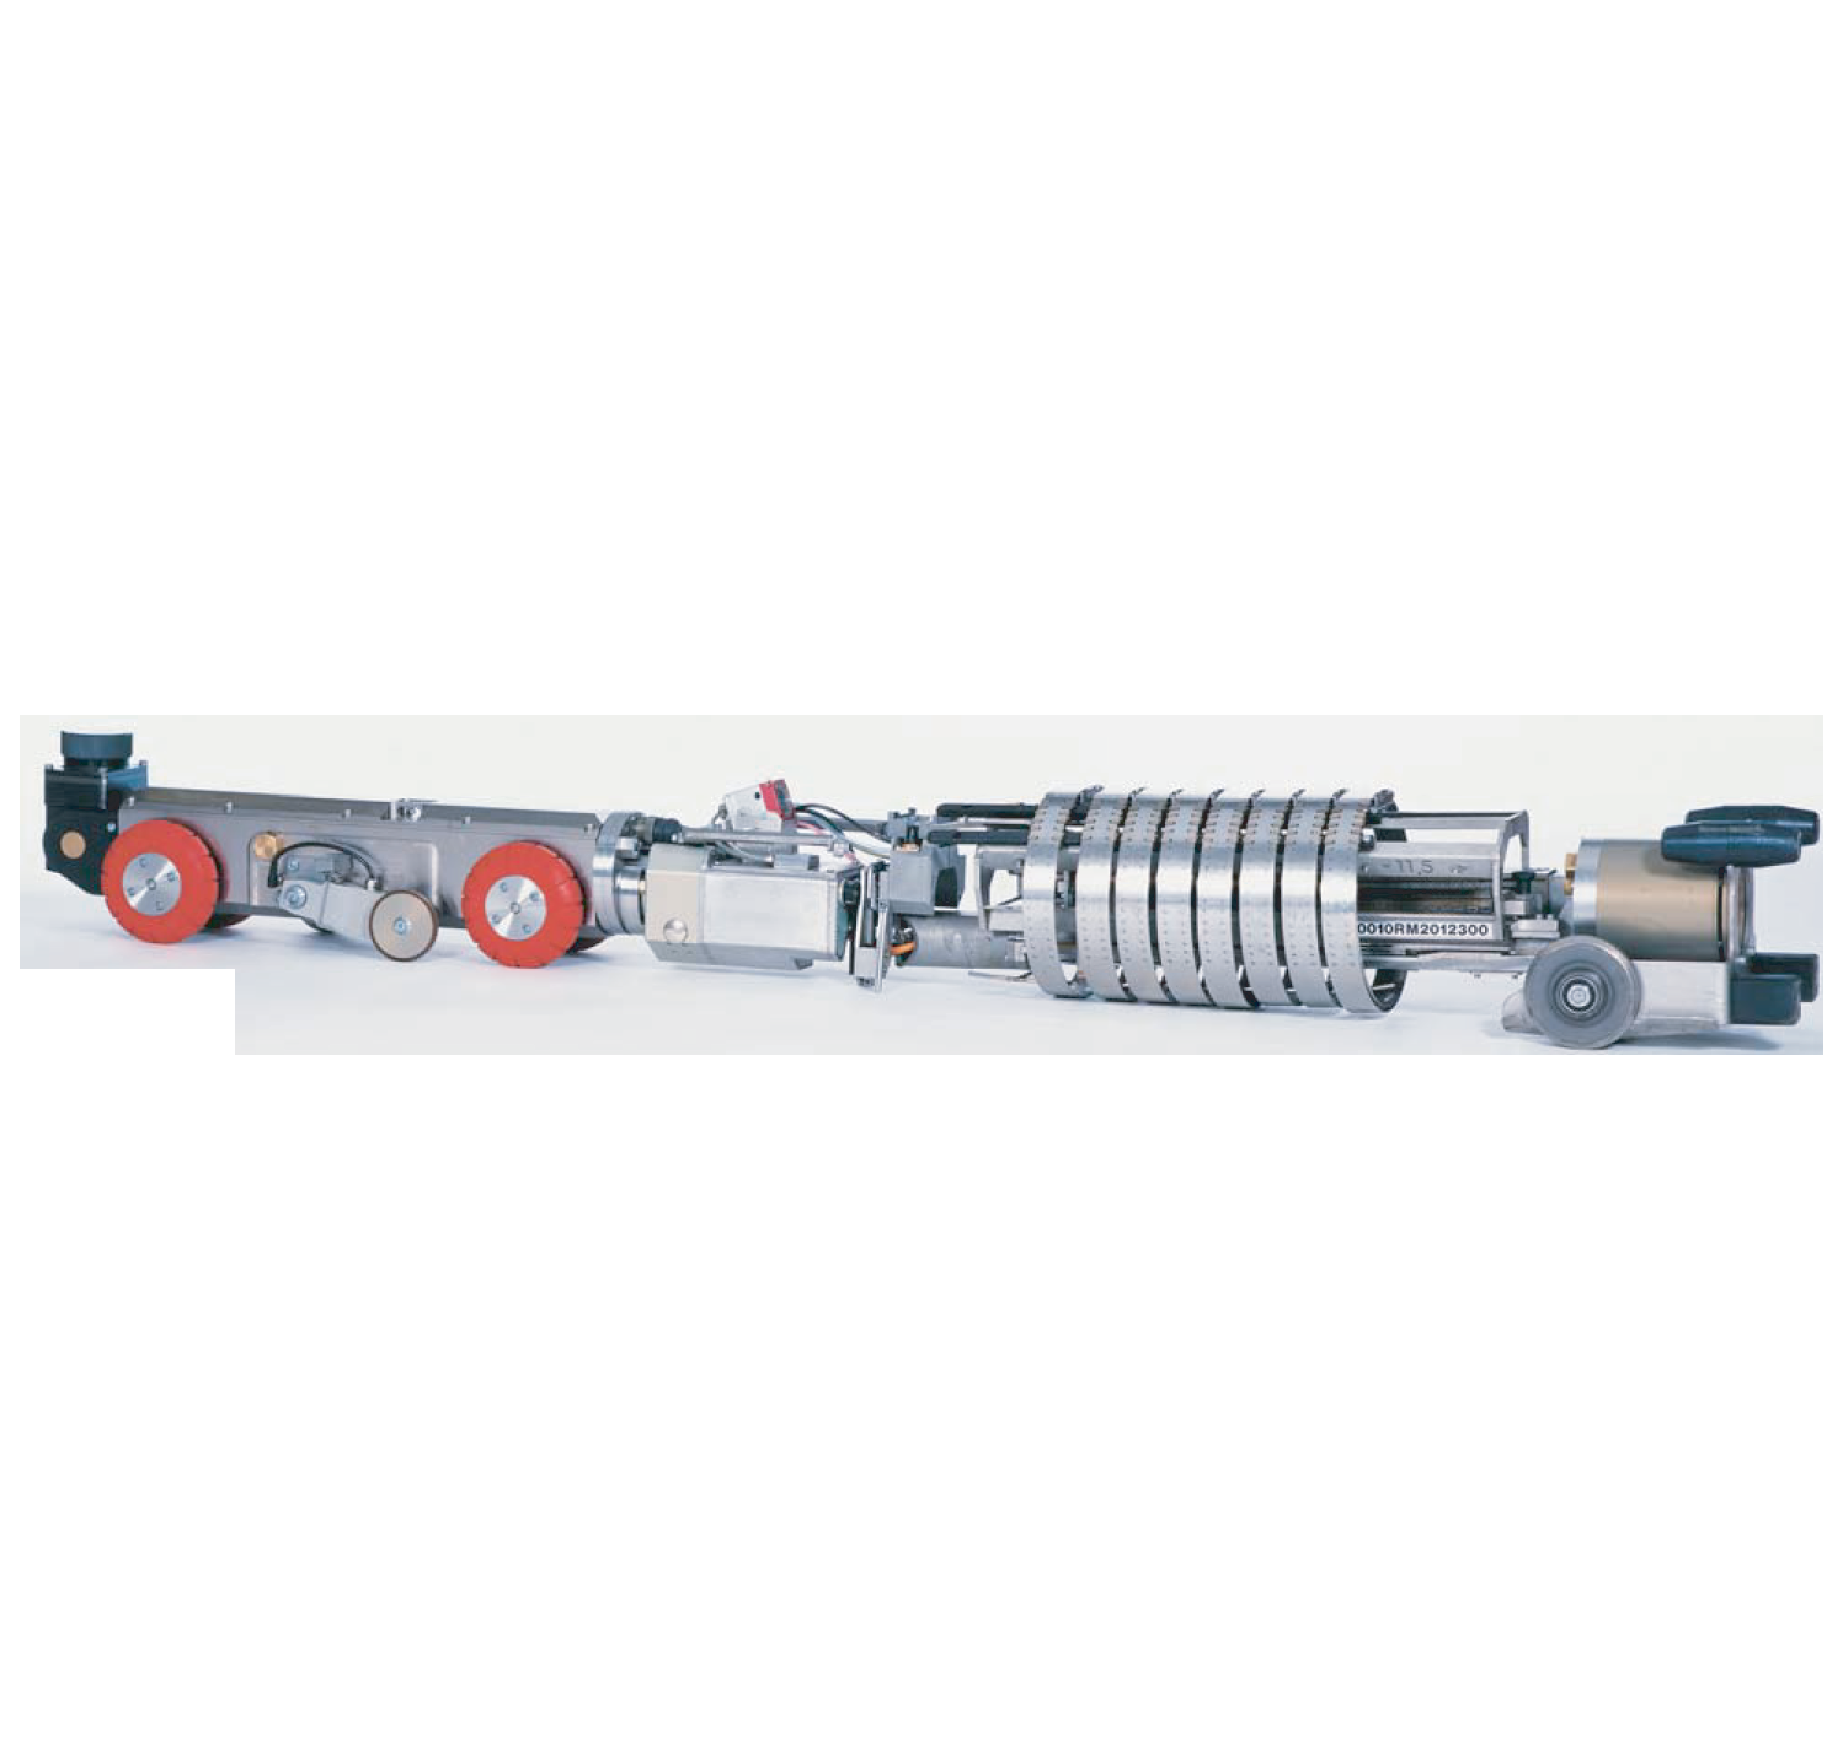
\includegraphics[width=\linewidth]{robot_photo.pdf}
\end{marginfigure}


\subsection*{Présentation}
\ifprof
\else
L'objet de cette étude est un robot permettant la pose d'arceaux métalliques pour l'installation de réseaux souterrains de télécommunication par fibres optiques.
\fi
\begin{obj}
En fin des mouvements des bras, on doit avoir $\delta=14\degres$ et $\dot{\delta}\leq 50\degres.\text{s}^{-1}$.
\end{obj}
%On donne le diagramme des exigences partiel du systèmes ci-dessous.
%
%\begin{center}
%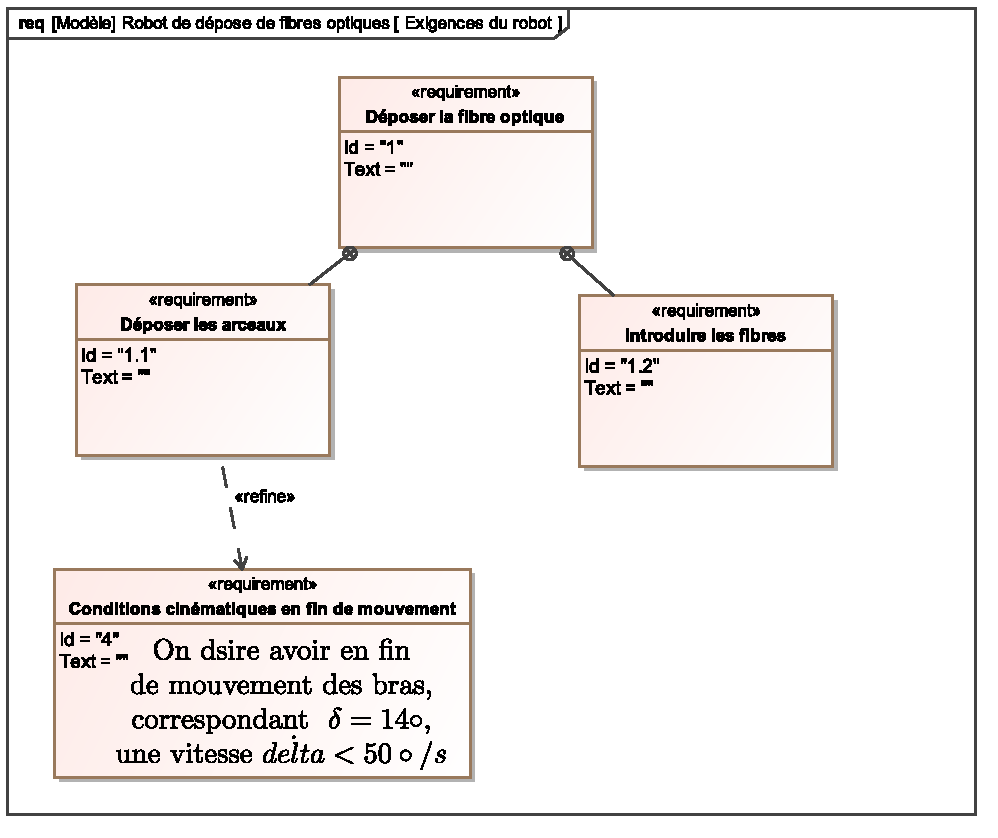
\includegraphics[width=\linewidth]{req_robot.pdf}
%\end{center}
\ifprof
\else


\begin{marginfigure}
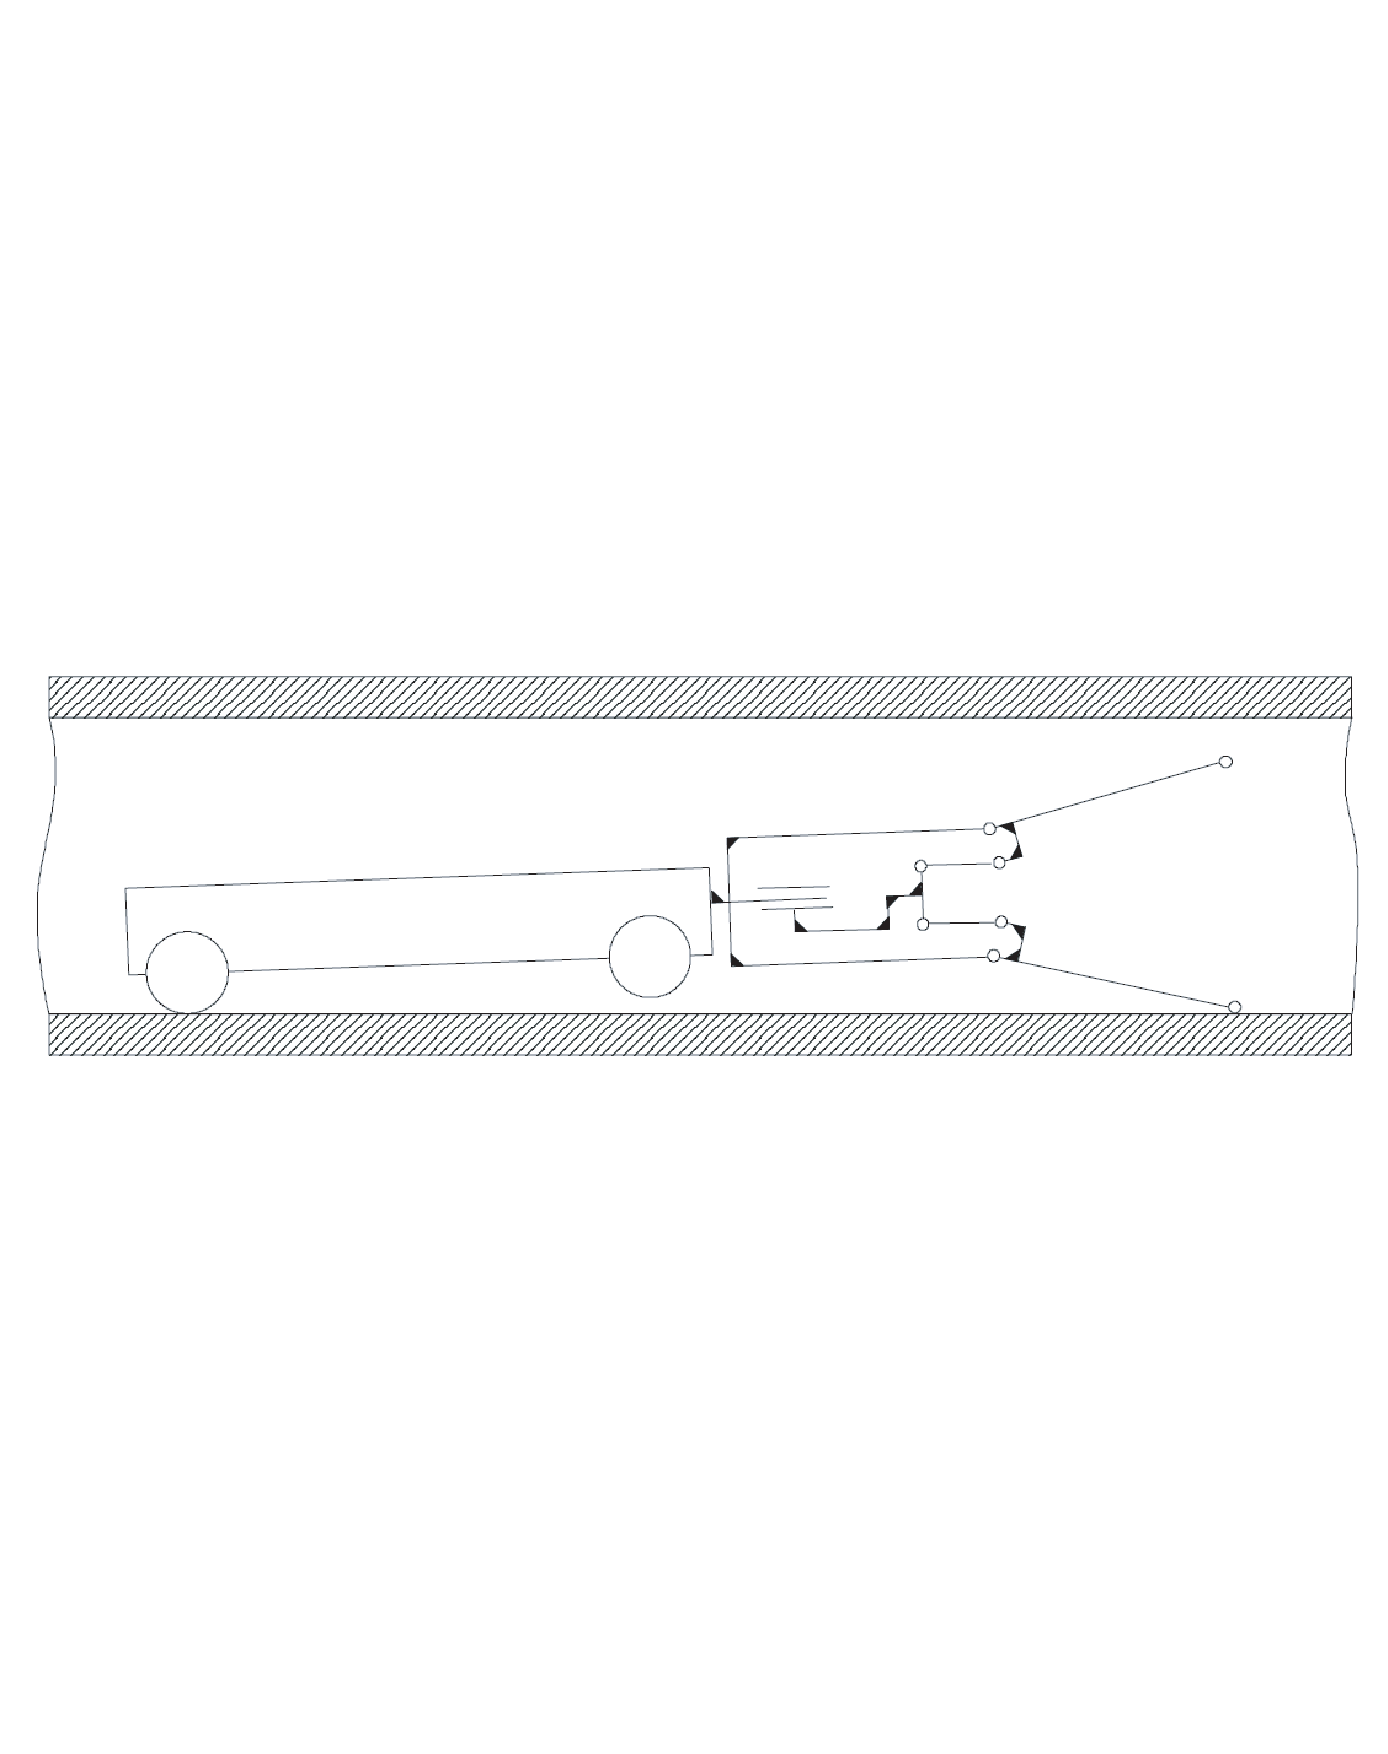
\includegraphics[width=\linewidth]{chariot_centrage1.pdf}
\end{marginfigure}


De façon à pouvoir dérouler les arceaux métalliques, le chariot est centré dans la canalisation à l'aide de quatre bras actionnés par un vérin hydraulique.


Afin de valider le choix du vérin, et donc sa puissance, il faut déterminer l'action $F$ du vérin
qui permettra au robot de se positionner correctement dans la canalisation.
%À l'instant où un anneau métallique doit être installé, les roues du train arrière sont bloquées par rapport au chariot. 
Sous l'effet
d'un vérin, les bras inférieurs vont soulever le
robot qui va pivoter sur son train arrière. La fin
du positionnement sera assurée lorsque les
roulettes des bras supérieurs viendront en
contact avec la paroi de la canalisation.
À un instant $t$, le système est modélisé selon le schéma ci-dessous :


\begin{marginfigure}
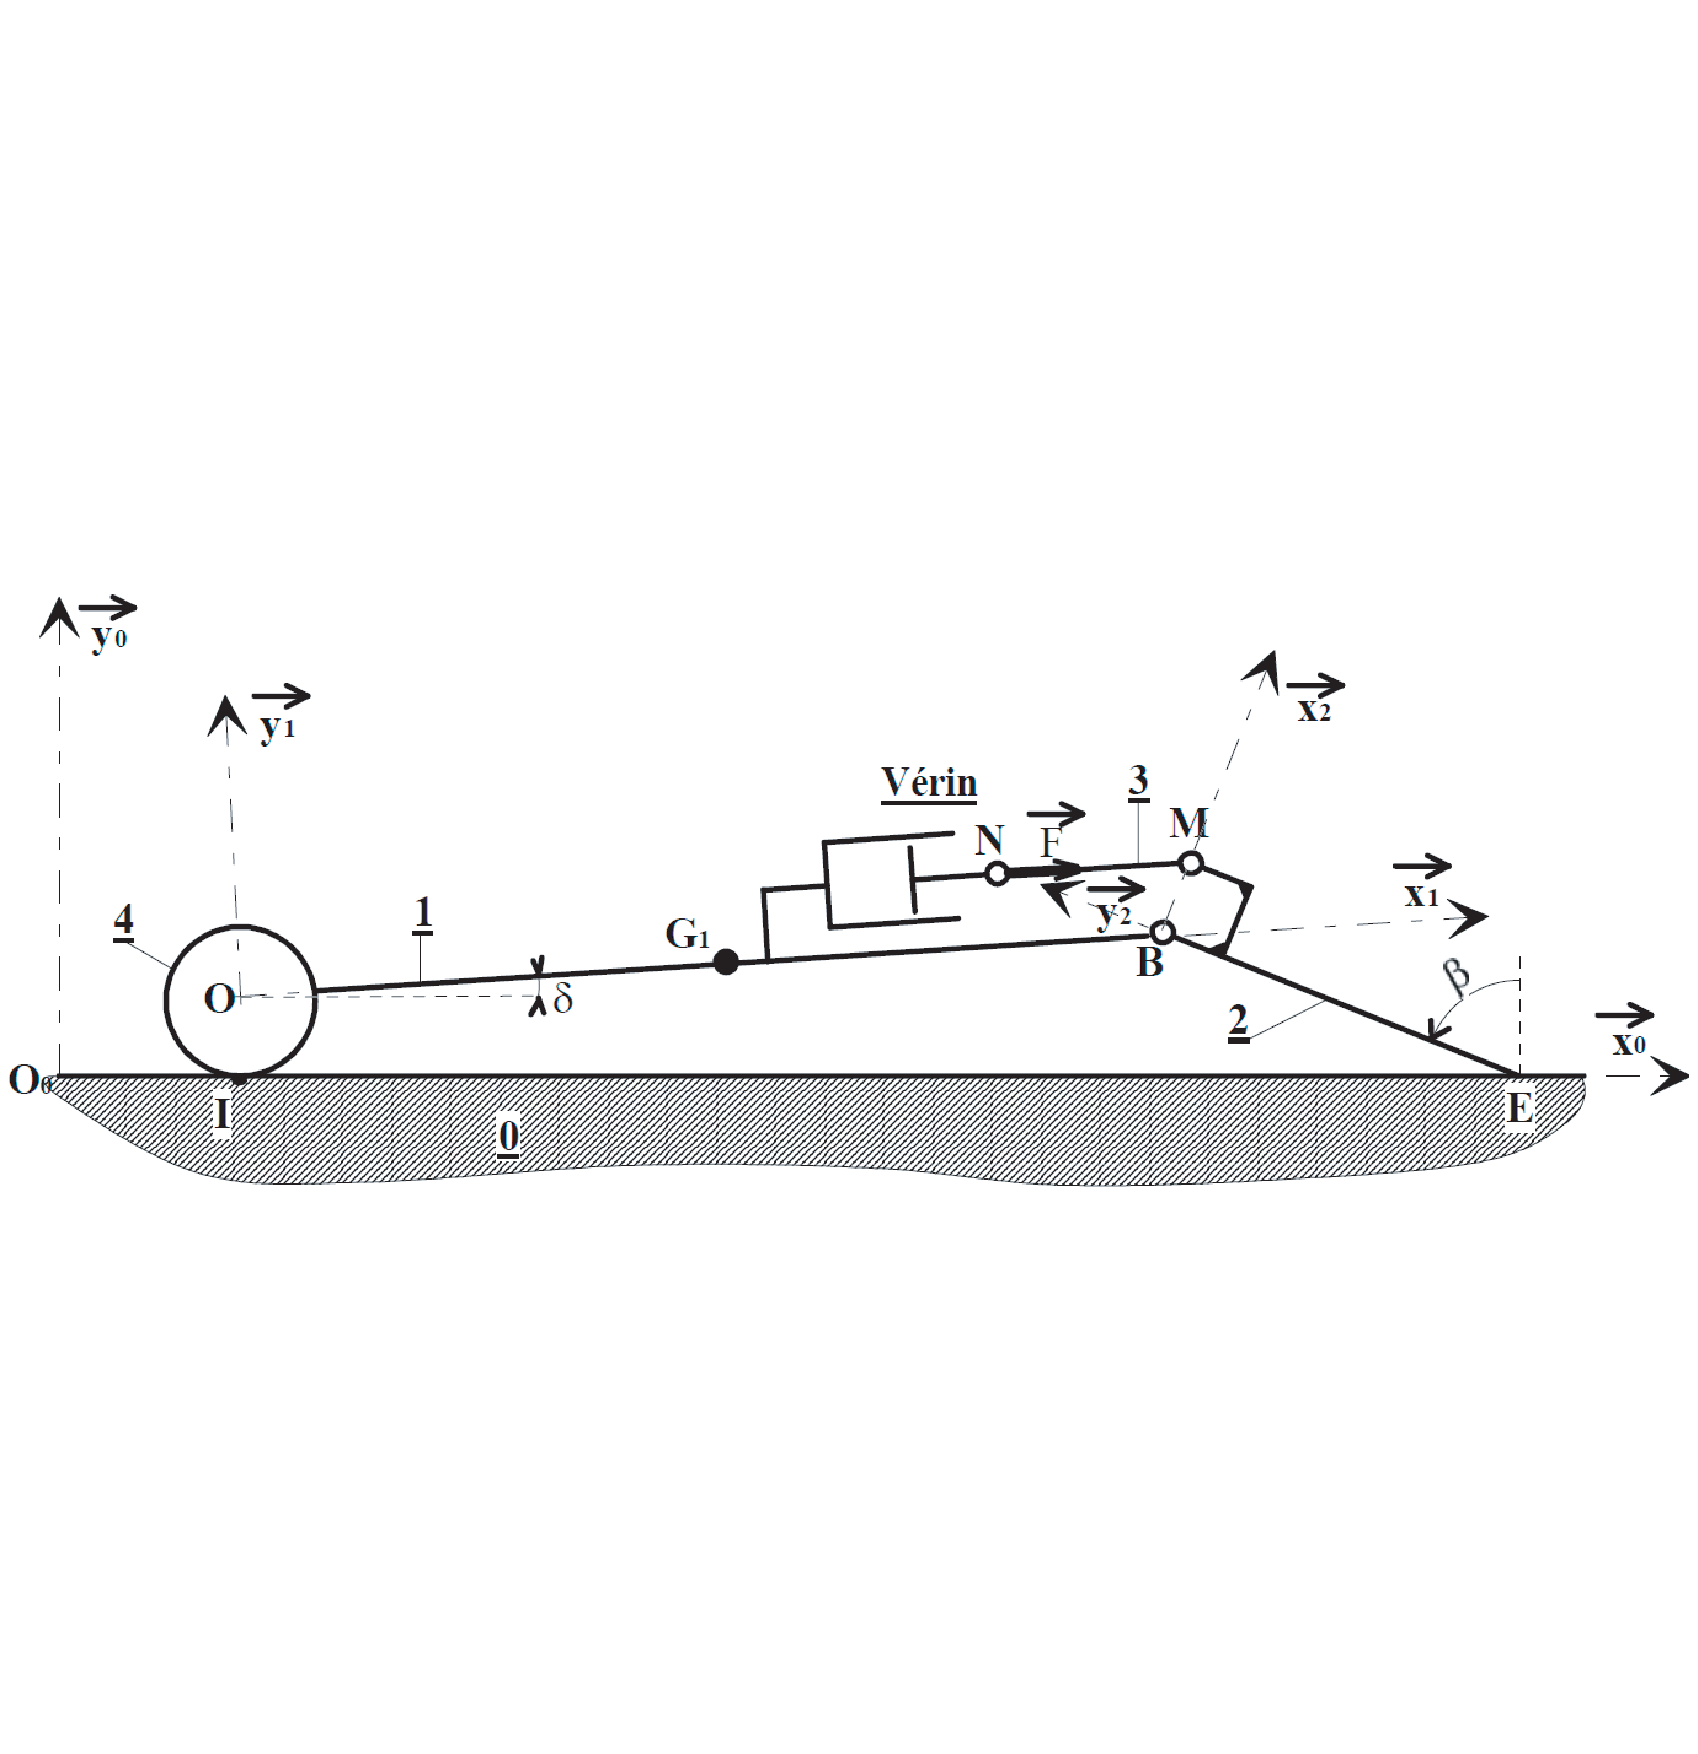
\includegraphics[width=0.9\linewidth]{chariot_centrage2.pdf}
%\caption{Modélisation du robot \label{robot_model}}
\end{marginfigure}
\fi

\subsection*{Hypothèses}
\ifprof
\else

L'étude dynamique est à faire dans le plan de symétrie longitudinale du robot.

Le robot est modélisé par le schéma ci-dessus. Il comprend :
\begin{itemize}
\item une tige \textbf{1} de longueur $OB=L_1$, de section négligeable, de masse $m_1$, et de centre d'inertie $G_1$, tel que $\overrightarrow{OG_1}=\frac{L_1}{2}\overrightarrow{x_1}$;
\item une roue $4$, de centre $O$, de rayon $R = \SI{0,07}{m}$, de masse négligeable, qui
correspond au train arrière. Cette roue est en liaison encastrement avec \textbf{1};
\item un bras \textbf{2} constitué de deux éléments $BE$ et $BM$ tels que $\overrightarrow{BE}=-a\overrightarrow{y_2}$ et $\overrightarrow{BM}=b\;\overrightarrow{x_2}$, de section et de masse négligeables;
\item une biellette \textbf{3} ($NM$) de masse négligeable et dont la direction au cours
du mouvement est sensiblement celle de la tige $1$;
\item un vérin hydraulique de masse négligeable.
\end{itemize}

 En $I$, le contact entre la roue \textbf{4} et la paroi \textbf{0} se fait par roulement sans glissement.

 En $E$, le contact entre le bras \textbf{2} et la paroi \textbf{0} se fait sans frottement.

Toutes les autres liaisons sont considérées sans frottement.

 L'action $\overrightarrow{F}$ du vérin sur la biellette $3a$, à chaque instant, pour direction $\overrightarrow{x_1}$ : 
$\overrightarrow{F} = F \overrightarrow{x_1}.$

\fi

\subsection*{Repères et paramétrage}
\ifprof
\else

\begin{itemize}
\item $R_0\quadruplet{O_0}{\overrightarrow{x_0}}{\overrightarrow{y_0}}{\overrightarrow{z_0}}$, repère associée à la canalisation $O$ et supposé galiléen.
\item $R_1\quadruplet{O}{\overrightarrow{x_1}}{\overrightarrow{y_1}}{\overrightarrow{z_1}}$, repère associé à la tige $1$.
\item $R_2\quadruplet{O}{\overrightarrow{x_2}}{\overrightarrow{y_2}}{\overrightarrow{z_2}}$, repère associé au bras $2$.
\item $\delta=\couple{\overrightarrow{x_0}}{{x_1}}=\couple{\overrightarrow{y_0}}{{y_1}}$.
\item $\beta=\couple{\overrightarrow{x_0}}{{x_2}}=\couple{\overrightarrow{y_0}}{{y_2}}$.
\end{itemize}

\fi
\subsection*{Cahier des charges}

\ifprof
\else
On désire avoir en fin de mouvement des bras, correspondant à $\delta=14^{\circ}$, une vitesse $\dot{\delta}$ inférieur à $50^{\circ}/s$
\fi
\subsection*{Modélisation dynamique}

\question{Donner l'expression de l'énergie cinétique galiléenne de l'ensemble $\Sigma=\left\{1+2+3+4\right\}$, puis la calculer.}
\ifprof
\begin{corrige}
Pour calculer l'énergie cinétique de l'ensemble seule la masse de la tige 1 est prise en compte.
$
2\;E_c(\Sigma/R_0)=\torseurci{\Sigma}{R_0}\otimes \torseurcin{V}{\Sigma}{R_0}$
$=\torseurl{\overrightarrow{\Omega}(1/0)}{\overrightarrow{V}(G_1,1/0)}{G_1}\otimes \torseurl{m_1\;\overrightarrow{V}(G_1,1/0)}{\overrightarrow{\sigma}(G_1,1/0)}{G_1}$
$=m_1\;\left(\overrightarrow{V}(G_1,1/0)\right)^2+\overrightarrow{\sigma}(G_1,1/0)\cdot \overrightarrow{\Omega}(1/0). 
$

\begin{itemize}
\item Vecteur de taux de rotation de $1$ par rapport à $0$ : $
\overrightarrow{\Omega}(1/0)=\dot{\delta}\;\overrightarrow{z_0}.
$

\item Vitesse du point $G_1$ appartenant à $1$ par rapport à $0$ : $
\overrightarrow{V}(G_1,1/0)=\overrightarrow{V}(I,1/0)+\overrightarrow{G_1I_1}\wedge\overrightarrow{\Omega}(1/0)$
$=-\left(R\;\overrightarrow{y_0}+\frac{L_1}{2}\overrightarrow{x_1}\right)\wedge\dot{\delta}\overrightarrow{z_0}$
$=-R\;\dot{\delta}\;\overrightarrow{x_0}+\frac{L_1}{2}\;\dot{\delta}\overrightarrow{y_1}$.


\item Caractéristiques d'inertie de la tige 1 : la tige $1$ supposée unidimensionnelle présente naturellement des symétries matérielles suivant des plans contenant $\overrightarrow{x_1}$. Les produits d'inertie sont donc nuls. Le moment d'inertie en $G_1$ suivant $\overrightarrow{z_0}$ est $C_1=\frac{m_1\;L_1^2}{12}$.

\item Moment cinétique en $G_1$ de 1 par rapport à 0 : $
\overrightarrow{\sigma}(G_1,1/0)=\overline{\overline{I}}_{G_1}(1)\cdot \overrightarrow{\Omega}(1/0)=\frac{m_1\;L_1^2}{12}\dot{\delta}\;\overrightarrow{z_0}
$.

\item On en déduit $E_c(1/0)$ :
$E_c(\Sigma/0)=E_c(1/0)$
$=\frac{1}{2}\;m_1\;\dot{\delta}^2\left(R^2+\frac{L_1^2}{4}+R\;L_1\;\sin\delta\right)+\frac{m_1\;L_1^2}{12}\;\dot{\delta}^2$

$=\frac{1}{2}\;m_1\;\dot{\delta}^2\left(R^2+\frac{L_1^2}{3}+R\;L_1\sin\delta\right)$.
\end{itemize}
\end{corrige}
\else
\fi

\question{Donner la puissance galiléenne des actions mécaniques extérieures agissant sur $\Sigma$.}
\ifprof
\begin{corrige}
$
\mathcal{P}(\text{ext}\rightarrow \Sigma/0)=\mathcal{P}(\text{pesanteur}\rightarrow \Sigma/0)+\mathcal{P}(\text{contact en E}\rightarrow \Sigma/0)+\mathcal{P}(\text{contact en I}\rightarrow \Sigma/0)
$

\begin{itemize}
\item Actions de la pesanteur :

$
\mathcal{P}(\text{\text{pes}}\rightarrow \Sigma/0)=\mathcal{P}(\text{\text{pes}}\rightarrow 1/0)=\torseurstat{T}{\text{pes}}{1}\otimes \torseurcin{V}{1}{0}
=\torseurl{-m_1\;g\;\overrightarrow{y_0}}{\overrightarrow{0}}{G_1}\otimes \torseurl{\overrightarrow{\Omega}(1/0}{\overrightarrow{V}(G_1,1/0)}{G_1}\\
=-m_1\;g\;\overrightarrow{y_0}\cdot\overrightarrow{V}(G_1,1/0)=-m_1\;g\frac{L_1}{2}\dot{\delta}\;\cos\delta.
$

\item Actions du contact en I entre $0$ et $4$ (\textit{le contact se fait par roulement sans glissement}) :

$
\mathcal{P}(\mbox{contact en I}\rightarrow \Sigma/0)=\torseurstat{T}{0}{4}\otimes \torseurcin{V}{4}{0}
=\torseurl{\overrightarrow{R}_{04}}{\overrightarrow{0}}{I}\otimes \torseurl{\overrightarrow{\Omega}(4/0)}{\overrightarrow{0}}{I}=0.
$

\item Actions du contact en E entre $0$ et $2$ (\textit{le contact se fait sans frottement}) :

$
\mathcal{P}(\mbox{contact en E}\rightarrow \Sigma/0)=\torseurstat{T}{0}{2}\otimes \torseurcin{V}{4}{0}
=\torseurl{R_{02}\;\overrightarrow{y_0}}{\overrightarrow{0}}{E}\otimes \torseurl{\overrightarrow{\Omega}(2/0)}{\overrightarrow{V}(E,2/0)}{E}=R_{02}\;\overrightarrow{y_0}\cdot\overrightarrow{V}(E,2/0)=0.
$



\end{itemize}
\end{corrige}
\else
\fi



\question{Donner la puissance intérieure à $\Sigma$.}
\ifprof
\begin{corrige}
\begin{itemize}
\item Les liaisons sont supposées comme parfaites donc : $\pint{1}{2}{Pivot} =\pint{1}{3}{Pivot Gl.} =\pint{3}{2}{Pivot} =0$.


\item Action du vérin entre 1 et 3 :

$ 
\pint{1}{3}{Vérin}=\torseurstat{T}{1}{3}\otimes \torseurcin{V}{3}{1}
=\torseurl{\overrightarrow{F}}{\overrightarrow{0}}{N}\otimes \torseurl{\overrightarrow{0}}{\overrightarrow{V}(N,3/1)}{N}
=F\;\overrightarrow{V}(N,3/1)\cdot\overrightarrow{x_1}.
$
%
%En appliquant la relation d'équiprojectivité au solide 1, on obtient :
%
%$
%\overrightarrow{V}(N,3/1)\cdot\overrightarrow{MN}=\overrightarrow{V}(M,3/1)\cdot\overrightarrow{MN}.
%$

En considérant que $\overrightarrow{MN}$ est porté par $\overrightarrow{x_1}$ (hypothèse faite dans l'énoncé), on obtient :

$
\overrightarrow{V}(N,3/1)\cdot\overrightarrow{x_1}$ 
$=\overrightarrow{V}(M,3/1)\cdot\overrightarrow{x_1}$
$=\left(\overrightarrow{V}(M,3/2)+\overrightarrow{V}(M,2/1)\right)\cdot\overrightarrow{x_1}$
$=\left(\vect{0}+\overrightarrow{V}(B,2/1) + \vect{MB}\wedge \vecto{2}{1}\right)\cdot\overrightarrow{x_1}$
$=\left(-b\vect{x_2} \wedge \left( \dot{\beta} - \dot{\delta}\right)\vect{z_0}\right)\cdot\overrightarrow{x_1}$
$=b\;\left(\dot{\beta}-\dot{\delta}\right)\cdot\overrightarrow{y_2}\cdot\overrightarrow{x_1}=-b\;\left(\dot{\beta}-\dot{\delta}\right)\sin(\beta-\delta)$.


On en déduit : $ \pint{1}{3}{Vérin}=-F\;b\;\left(\dot{\beta}-\dot{\delta}\right)\sin(\beta-\delta) $.

\end{itemize}
\end{corrige}
\else
\fi

\question{Appliquer le théorème de l'énergie cinétique à $\Sigma$ pour déterminer l'équation de mouvement donnant une relation entre $F$, $\delta$, et $\beta$.}
\ifprof
\begin{corrige}
On applique alors le théorème de l'énergie cinétique à $\Sigma$ par rapport au référentiel galiléen $R_0$ :

$
\frac{\dd }{\dd t}(E_c(\Sigma/R_0))=\mathcal{P}(\text{ext}\rightarrow \Sigma/0)+\mathcal{P}_\text{int}( \Sigma).
$

Or, $
\frac{\dd }{\dd t}(E_c(\Sigma/R_0))$ 
$=\frac{\dd }{\dd t}\left[\frac{1}{2}\;m_1\;\dot{\delta}^2\left(R^2+\frac{L_1^2}{3}+R\;L_1\sin\delta\right)\right]$
$=m_1\;\dot{\delta}\left[\ddot{\delta}\left(R^2+\frac{L_1^2}{3}+R\;L_1\sin\delta\right)+\frac{1}{2}\dot{\delta}^2\;R\;L_1\cos\delta\right]$.


Ainsi on obtient, l'équation :


$
\boxed{
m_1\;\dot{\delta}\left[\ddot{\delta}\left(R^2+\frac{L_1^2}{3}+R\;L_1\sin\delta\right)+\frac{1}{2}\dot{\delta}^2\;R\;L_1\cos\delta\right]
=-F\;b\;\left(\dot{\beta}-\dot{\delta}\right)\sin(\beta-\delta)-m_1\;g\frac{L_1}{2}\dot{\delta}\;\cos\delta.
}
$

\end{corrige}
\else
\fi

\ifprof
\else
\ifcolle
\else
\noindent
\marginnote[-5cm]{
\begin{solution}
\begin{enumerate}
\item  $E_c=\frac{1}{2}\;m_1\;\dot{\delta}^2\left(R^2+\frac{L_1^2}{3}+R\;L_1\sin\delta\right)$.
\item  $ \mathcal{P}(\text{\text{ext}}\rightarrow \Sigma/0)= -m_1\;g\frac{L_1}{2}\dot{\delta}\;\cos\delta $.
\item  $ \mathcal{P}_{\text{int}}\left( \Sigma\right)=-F\;b\;\left(\dot{\beta}-\dot{\delta}\right)\sin(\beta-\delta) $
\item $m_1\;\dot{\delta}\left[\ddot{\delta}\left(R^2+\frac{L_1^2}{3}+R\;L_1\sin\delta\right)+\frac{1}{2}\dot{\delta}^2\;R\;L_1\cos\delta\right]
=-F\;b\;\left(\dot{\beta}-\dot{\delta}\right)\sin(\beta-\delta)-m_1\;g\frac{L_1}{2}\dot{\delta}\;\cos\delta $.
\end{enumerate} 
\end{solution}}
\fi
\fi



Des simulations pour différentes valeurs de $F$ donnent les diagrammes (figure suivante) représentant l'évolution de $\delta$ en fonction du temps.

\question{Pour chaque diagramme, analyser le comportement du robot. Déterminer les vitesses $\dot{\delta}$ en fin de course. En déduire les valeurs de F respectant le cahier des charges.}
\ifprof
\begin{corrige}
\begin{itemize}
\item \textbf{$F=\SI{700}{N}$} : le régime est fortement oscillant. Le système ne parvient pas à soulever
le robot jusqu'à $14^{\circ}$. Celui-ci se comporte comme un oscillateur non
amorti (le modèle est considéré sans frottement).

Cette valeur de l'effort n'est pas satisfaisante.

\item \textbf{$F=\SI{750}{N}$} : le système atteint les $14^{\circ}$. La pente à l'accostage vaut environ $37.5^{\circ}/s$
ce qui est raisonnable vis-à-vis du cahier des charges. Cependant, le
modèle utilisé pour trouver ce résultat utilise des liaisons parfaites,
sans frottement. L'effort de $\SI{700}{N}$ étant insuffisant avec ce modèle
parfait, il est possible qu'un effort de $\SI{750}{N}$ devienne insuffisant en
réalité.

Cette valeur est théoriquement satisfaisante mais l'écart entre modèle
et réalité risque de modifier la conclusion.

\item \textbf{$F=\SI{800}{N}$} : Le système atteint les $14^{\circ}$ La pente à l'accostage vaut environ $45^{\circ}/s$ ce
qui est inférieur à la limite de $50^{\circ}/s$ imposée par le cahier des
charges. L'effort est $15\%$ supérieur à la valeur minimale nécessaire
pour atteindre les $14^{\circ}$ ce qui semble une marge suffisante pour vaincre
les frottements non pris en compte dans le modèle.

Cette valeur est satisfaisante.

\item \textbf{$F=\SI{950}{N}$} : Le système atteint les $14^{\circ}$. La pente à l'accostage vaut environ $75^{\circ}/s$ ce
qui est supérieur à la limite de $50^{\circ}/s$ imposée par le cahier des
charges.

Cette valeur de l'effort n'est pas satisfaisante.
\end{itemize}

\begin{center}
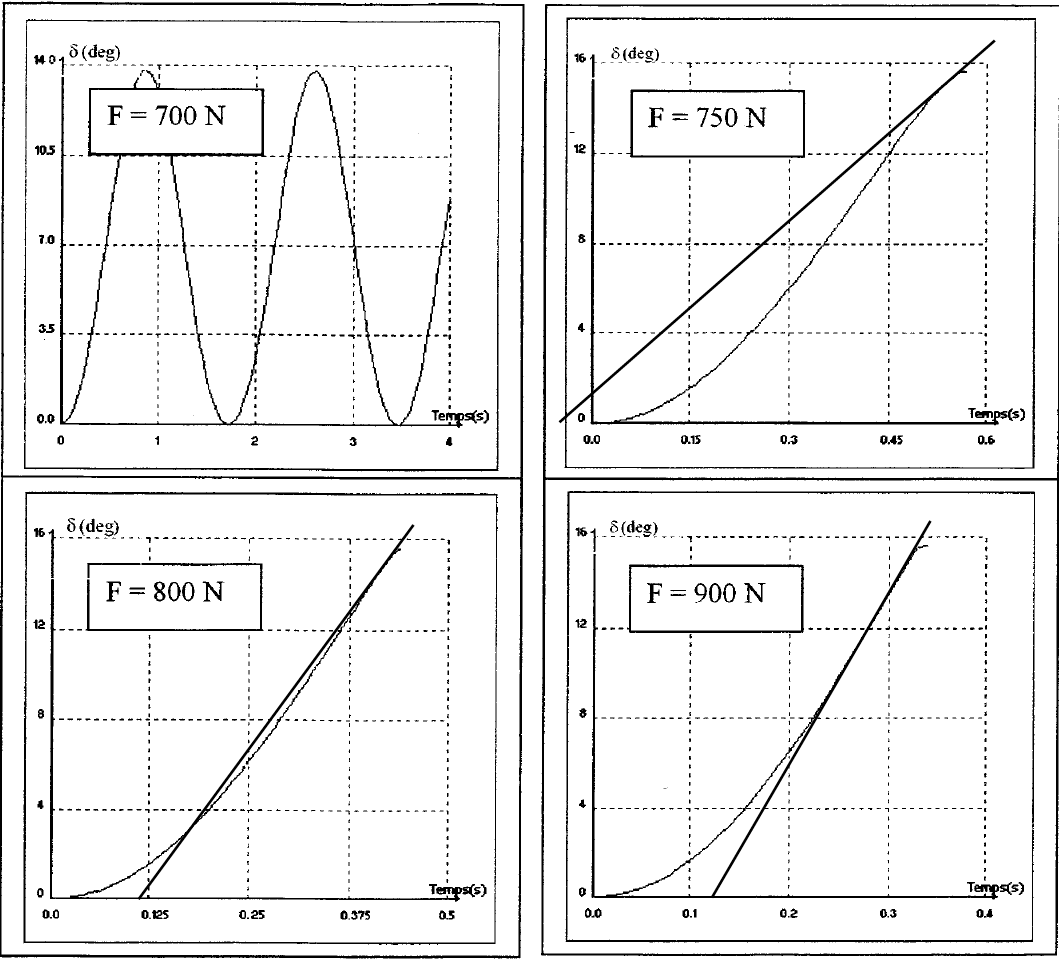
\includegraphics[width=1.0\textwidth]{courbes_simulation_corrige.png}
\end{center}

\end{corrige}
\else
\fi

\ifprof
\else
\begin{marginfigure}
\centering

\includegraphics[width=3cm]{Cy_05_01_TD_04_RobotFibre_qr}
\end{marginfigure}
\fi


\ifprof
\else

%\begin{figure}[!ht]
\begin{center}
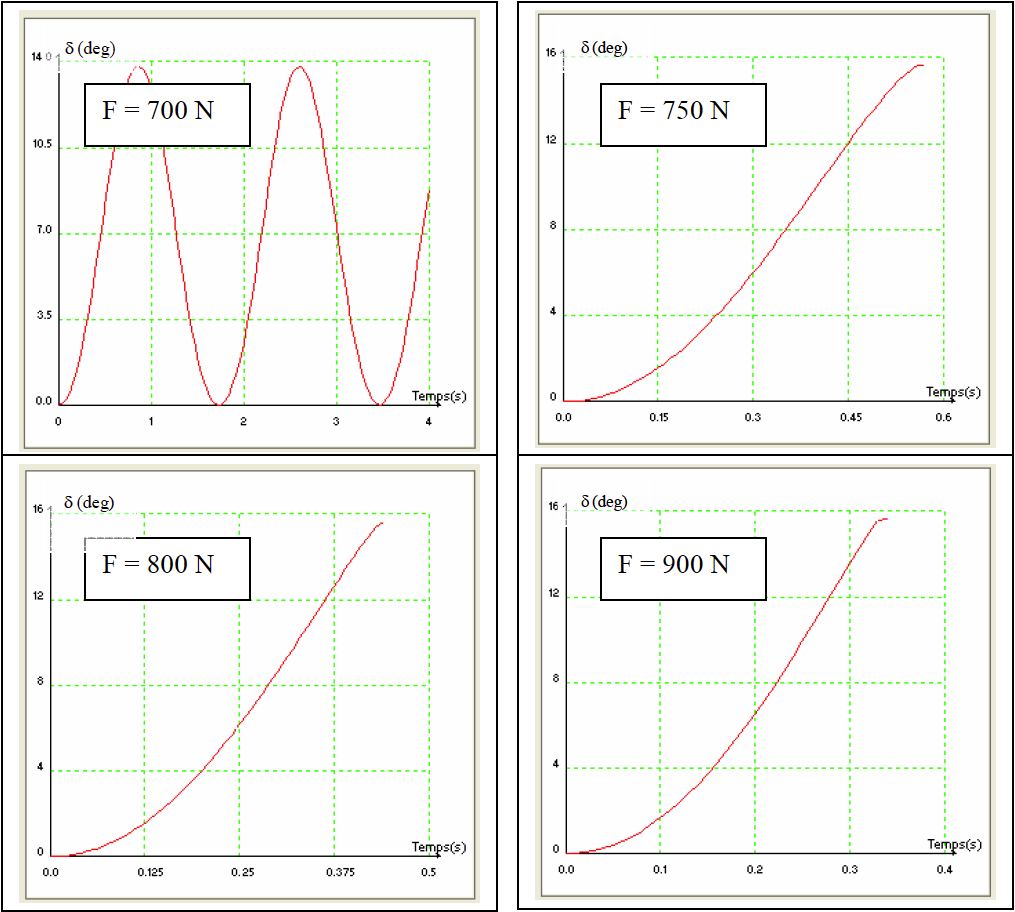
\includegraphics[width=.8\linewidth]{courbes_simulation.png}
%\caption{Résultats de la simulation dynamique du système \label{simulation_dynamique}}
\end{center}
%\end{figure}
\fi

